\justifying \small 

\textcolor{orange}{\#include <stdio.h>} \textcolor{gray}{/* Hello 
 * World program
 **/} \textcolor{cyan}{void} \textcolor{white}{main} 
\textcolor{magenta}{(} \textcolor{magenta}{)} \textcolor{magenta}{\{} \textcolor{gray}{// declara una variable "asd"*/} 
\textcolor{cyan}{int} \textcolor{white}{d} \textcolor{yellow}{=} \textcolor{green}{-.5e-1} 
\textcolor{yellow}{*} \textcolor{green}{521} \textcolor{magenta}{;} \textcolor{red}{\$} 
\textcolor{white}{printf} \textcolor{magenta}{(} \textcolor{green}{"resultado: \%d"} \textcolor{magenta}{,} 
\textcolor{white}{d} \textcolor{magenta}{)} \textcolor{magenta}{;} \textcolor{cyan}{return} 
\textcolor{green}{0} \textcolor{magenta}{;} \textcolor{magenta}{\}} \textcolor{red}{\$} 
\textcolor{red}{\textbackslash} \textcolor{cyan}{void} \textcolor{white}{main} \textcolor{magenta}{(} 
\textcolor{magenta}{)} \textcolor{magenta}{\{} \textcolor{gray}{// declara una variable "asd"*/} \textcolor{cyan}{int} 
\textcolor{white}{d} \textcolor{yellow}{=} \textcolor{green}{-.5e-1} \textcolor{yellow}{*} 
\textcolor{green}{521} \textcolor{magenta}{;} \textcolor{red}{\$} \textcolor{white}{printf} 
\textcolor{magenta}{(} \textcolor{green}{"resultado: \%d"} \textcolor{magenta}{,} \textcolor{white}{d} 
\textcolor{magenta}{)} \textcolor{magenta}{;} \textcolor{cyan}{return} \textcolor{green}{0} 
\textcolor{magenta}{;} \textcolor{magenta}{\}} \textcolor{red}{\$} \textcolor{red}{\textbackslash} 
\textcolor{cyan}{void} \textcolor{white}{main} \textcolor{magenta}{(} \textcolor{magenta}{)} 
\textcolor{magenta}{\{} \textcolor{gray}{// declara una variable "asd"*/} \textcolor{cyan}{int} \textcolor{white}{d} 
\textcolor{yellow}{=} \textcolor{green}{-.5e-1} \textcolor{yellow}{*} \textcolor{green}{521} 
\textcolor{magenta}{;} \textcolor{red}{\$} \textcolor{white}{printf} \textcolor{magenta}{(} 
\textcolor{green}{"resultado: \%d"} \textcolor{magenta}{,} \textcolor{white}{d} \textcolor{magenta}{)} 
\textcolor{magenta}{;} \textcolor{cyan}{return} \textcolor{green}{0} \textcolor{magenta}{;} 
\textcolor{magenta}{\}} \textcolor{red}{\$} 



\begin{frame}{Histograma Tokens Usados} 
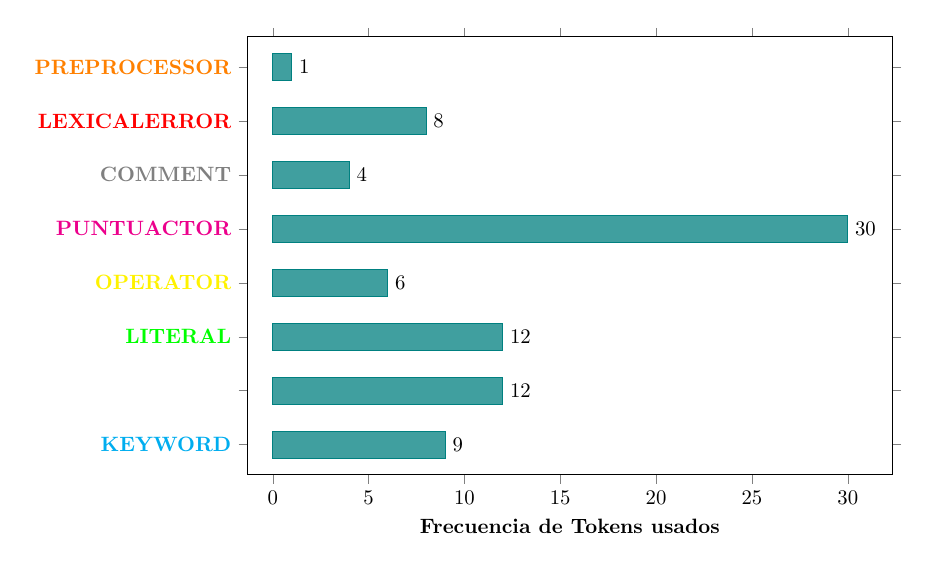
\begin{tikzpicture}[scale=0.75] % tamaño 
\begin{axis}[xbar,tick align=outside, 
    width=12.5cm,       % largo 
    height=9cm,       % altura 
    bar width={13pt},   % grosor linea 
    enlargelimits=0.08, % cercania a linea 
    nodes near coords, 
    nodes near coords align=horizontal, 
    point meta=x * 1, % The displayed number. 
    xlabel=\textbf{Frecuencia de Tokens usados}, 
    ytick={0,...,7}, 
    yticklabels={ 
        \textcolor{cyan}{\textbf{KEYWORD}},         % POSITION 0 
        \textcolor{white}{\textbf{IDENTIFIER}},     % POSITION 1 
        \textcolor{green}{\textbf{LITERAL}},        % POSITION 2 
        \textcolor{yellow}{\textbf{OPERATOR}},      % POSITION 3 
        \textcolor{magenta}{\textbf{PUNTUACTOR}},   % POSITION 4 
        \textcolor{gray}{\textbf{COMMENT}},         % POSITION 5 
        \textcolor{red}{\textbf{LEXICALERROR}},     % POSITION 6 
        \textcolor{orange}{\textbf{PREPROCESSOR}}   % POSITION 7 
    }] 
\addplot 
[draw=teal,fill=teal!75] 
coordinates {(9,0) (12,1) (12,2) (6,3) (30,4) (4,5) (8,6) (1,7)}; 
\end{axis}
\end{tikzpicture}
\end{frame}
